% Chapter 1

\chapter{Introduction} % Main chapter title

\label{Chapter1} % For referencing the chapter elsewhere, use \ref{Chapter1} 

%----------------------------------------------------------------------------------------

% Define some commands to keep the formatting separated from the content 
\newcommand{\keyword}[1]{\textbf{#1}}
\newcommand{\tabhead}[1]{\textbf{#1}}
\newcommand{\code}[1]{\texttt{#1}}
\newcommand{\file}[1]{\texttt{\bfseries#1}}
\newcommand{\option}[1]{\texttt{\itshape#1}}

%----------------------------------------------------------------------------------------

Currently, in the 21st century, computers have become ubiquitous in our everyday lives. Formerly mundane tasks like switching on/off light switches, vacuuming, counting objects, and accurately predicting sales, to safety-critical tasks like driving vehicles and trains are currently performed efficiently by computers. Now, efforts are being made to extend the capabilities of computer systems to perform intelligent tasks like disease detection, speech-to-text transcribing, anomaly detections that humans otherwise perform. However, the challenging part is transferring this knowledge to computers to perform such analysis and inference tasks. The approach humans use in learning is by transferring knowledge of a system to another related system. For example, humans can effortlessly differentiate between a cat and a dog in an image. This ability to differentiate is possible because specific characteristics are present in dogs but absent in cats, irrespective of their breeds. However, manually programming computers to make such differentiation will prove impractical or possibly amount to several lines of code. Likewise, it is unrealistic to manually program a computer to detect diseases in an image or make driving decisions in autonomous vehicles. 

These shortcomings for computers have motivated researchers to trial the use of machine learning techniques to for example allow computers to analyse and interpret objects in images or videos. An exciting use case in agriculture is training computers to monitor and detect plant leaf diseases or nutrient deficiencies through images. The use of computers to precisely monitor and give respective treatment to particular plants in plantations to get increased average yields and reduce operational farming costs is known as precision farming. 

Traditionally, disease detection techniques used to involve using naked eyes to visually inspect the leaves and branches of plants for any sign of infection. However, this plant health monitoring and disease detection method are time-consuming. For example, it is labour tasking and financially draining to inspect plant leaves spanning several hectares of land visually. Thanks to the advancements in the technological sector, researchers have shown the possibilities of plant health monitoring using machine learning techniques to classify plant leaves captured with RGB cameras and hyperspectral sensors as healthy or unhealthy. Unfortunately, one major challenge in using these technologies is the unavailability of enough datasets for model training.


\section{The Goal}
Plant diseases cause significant hindrances to the sustainability and profitability of agriculture \cite{harvey2014extreme}. In order to prevent the losses that come with diseases in plants, different methods have been developed to monitor and diagnose these diseases before they lead to a significant infestation. One such method is the use of established knowledge in molecular biology and immunology to precisely identify the causal agents of diseases in plants and develop treatments for eradicating them before they become catastrophic to the plants. However, such an approach requires experts in the disease domain to cut down the plants and perform tests to identify the specific disease affecting the plants. Moreover, this disease detection technique is invasive; it is likewise tedious and expensive \cite{wang2017automatic}.

These shortcomings in the traditional disease detection motivated researches in the direction of non-invasive plant disease detections using data from sensors like RGB, hyperspectral imaging and spectroscopy with machine learning algorithms \cite{mohanty2016using, ashourloo2016investigation, zhang2019deep}. The research results on the use of collected real-time data from plants with machine learning techniques showed promising results that are more accurate in plant disease detection and classification than domain experts in such fields, thereby potentially minimising costs for farmers. %[\cite{}]. 
Standard algorithms used for plant disease detection and classification tasks are linear regression, logistic regression, random forest, clustering, Gaussian models, decision trees (DT), Naïve Bayes (NB), K-nearest neighbours (KNN), and support vector machines (SVM) among others.


Despite the success of plant disease detection, using sensor data with classical machine learning algorithms was time-consuming due to manual feature extractions and not being robust enough for use on datasets containing variations from the original training dataset [cite]. Nevertheless, the learnings from ML laid a solid foundation for current researches in the direction of deep neural networks for automating the identification of disease from the data captured from sensors to allow precise plant treatment in a field. Furthermore, advancements in computer vision and artificial intelligence have led to solutions that were found to accurately solve complex decision-making tasks like yield forecasting \cite{liu2017computer}, plant recognition \cite{gao2017mobile}, and nutrition deficiency \cite{yi2020deep} in precision farming.

Deep neural networks require a large amount of image data with appropriate diversity representing different conditions that can likely occur to create a high-quality model for the trained tasks. However, capturing all the variability of conditions possible is a cumbersome task, hence the need to augment the existing dataset using computer vision and deep learning techniques to create robust image datasets for plant disease detection tasks in sugar beet. Particularly for sugar beet disease detection, there are no publicly accessible datasets and acquiring these datasets require several months and professionals to ensure the quality and diversity needed.
% [\cite{} papers that it took them months to get sugar beets dataset].

This thesis proposes the approach below to solve the problem of the lack of a public dataset for disease detection in sugar beet plants:
 \begin{itemize}
     \item Using image augmentation techniques to mask diseased areas in a plant on top of healthy areas in another plant. However, there should be a common disease occurrence in both plants.

 \end{itemize}


The results from creating these synthetic datasets will create an avenue for transferring knowledge in this domain to create more datasets for other plants, hence creating more than enough datasets for model training.

\section{Overview of Proposed Approach}
Our approach to artificial dataset creation is based on segmenting the leaf areas of the diseased and healthy plants from their background in the images and then concatenating the extracted diseased areas intelligently on the healthy leaf areas. First, we propose segmenting foreground and background leaf areas by converting the images to their respective HSV values to find the leaves’ upper and lower bound values. We then propose using Gaussian blur and morphological transformations to create binary masks of the leaf areas and the background and finally use boolean operations to create the new image. Furthermore, we propose bringing the infected areas of the diseased leaf foreground and then masking out healthy areas to become the background. Figure \ref{fig:my_arch} showcases a visual representation of the proposed artificial dataset creation pipeline. The values corresponding to the diseased areas are rotated and placed accordingly on the leaf areas of the sugar beet plants as shown in figure \ref{fig:my_arch}.

\begin{figure}[!htb]
    \centering
    \includegraphics[width=1\textwidth]{Figures/architecture.png}
    \caption{Sample image from the image folder}
    \label{fig:my_arch}
\end{figure}

With the resulting images from the previously proposed approach, we suggest potentially automating the process of creating more randomly unique datasets using generative adversarial neural networks (GAN) as depicted in figure \ref{fig:my_gan}. On a high level, GANs work by using two neural networks competing against each other to create synthetic datasets. As shown in figure \ref{fig:my_gan}, the neural generator network creates new synthetic image data, which are then fed to the discriminator neural network to ascertain how close the generated image is to the original images.

\section{Outline}
This chapter introduces the problem of plant health monitoring using machine learning techniques. First, it discusses the issue of not having enough datasets to train machine learning algorithms for plant health monitoring - particularly the lack of public datasets for disease detection in sugar beets. Then the chapter continues by shortly presenting the proposed approach to solving the lack of public dataset in sugar beet for disease detection tasks, highlighting the contributions of the thesis. The rest of the thesis is structured as follows.

\begin{itemize}
    
    \item \textbf{Chapter 2:} explains the relevant theories necessary for the experiment performed in this research. Furthermore, the chapter presents the related works to the thesis.

    \item \textbf{Chapter 3:} presents a high-level overview of the approach and its implementation

    \item \textbf{Chapter 4:} presents and discusses the results of the generated synthetic image datasets.

    \item \textbf{Chapter 5:} draws a conclusion of the thesis and recommendations for future work. 
    
\end{itemize}





% \subsection{Summary of Contributions}
% \subsection{Outline of thesis}
% \begin{figure}[!htb]
%     \centering
%     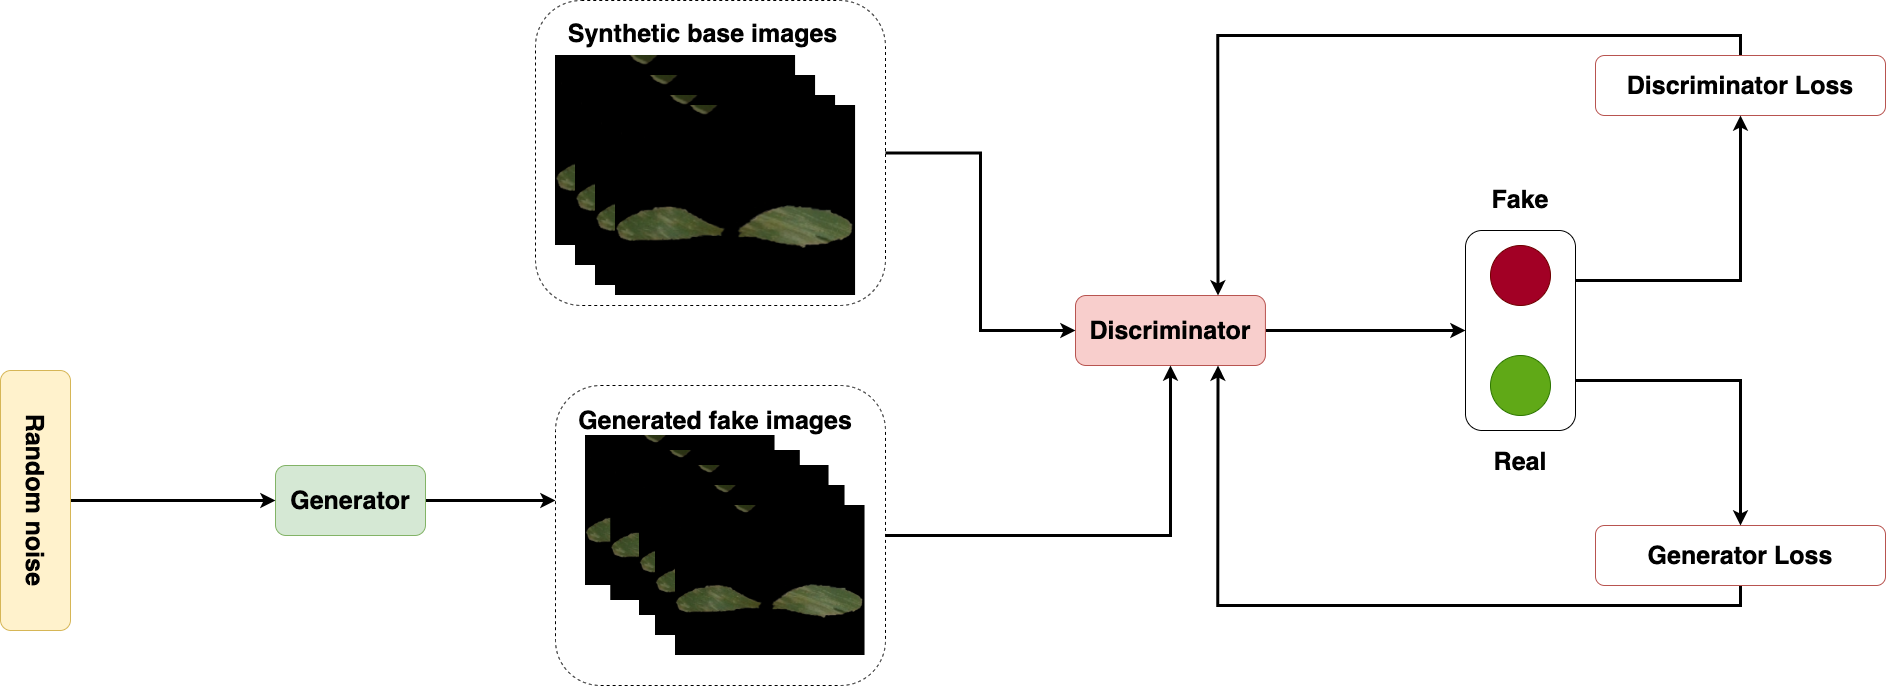
\includegraphics[width=1.2\textwidth]{Figures/gan.png}
%     \caption{Sample image from the image folder}
%     \label{fig:my_arch}
% \end{figure}
